\graphicspath{ {Approach/Images/} }


\chapter{General Word2vec Approach}
\label{cha:approach}

\section{Introduction}
In this chapter 

Joins of dataset
DiseaseMapping (generalization)
General approach 
Knn
KDtree
Deepwalk





\section{General Word2Vec}

Word2vec can be made distributed as the underlying idea is quite simplistic, it counts occurrences of n-grams. Counting occurrences based on labels, is a well known problem and is often solved by MapReduce algorithms. 


\section{Patient Classification}

As mentioned in section \ref{sec:word2vec}, a trained 2-layer neural network can be placed before another neural network and function as a lookup table. In this section, we discuss a possible neural network which allows us to further investigate the effectiveness of our word2vec approach to classify patients. More concrete: we should check if a better accuracy is acquired with the lookup table in front of the neural network or without. 


\begin{figure}[H]
	\centering
	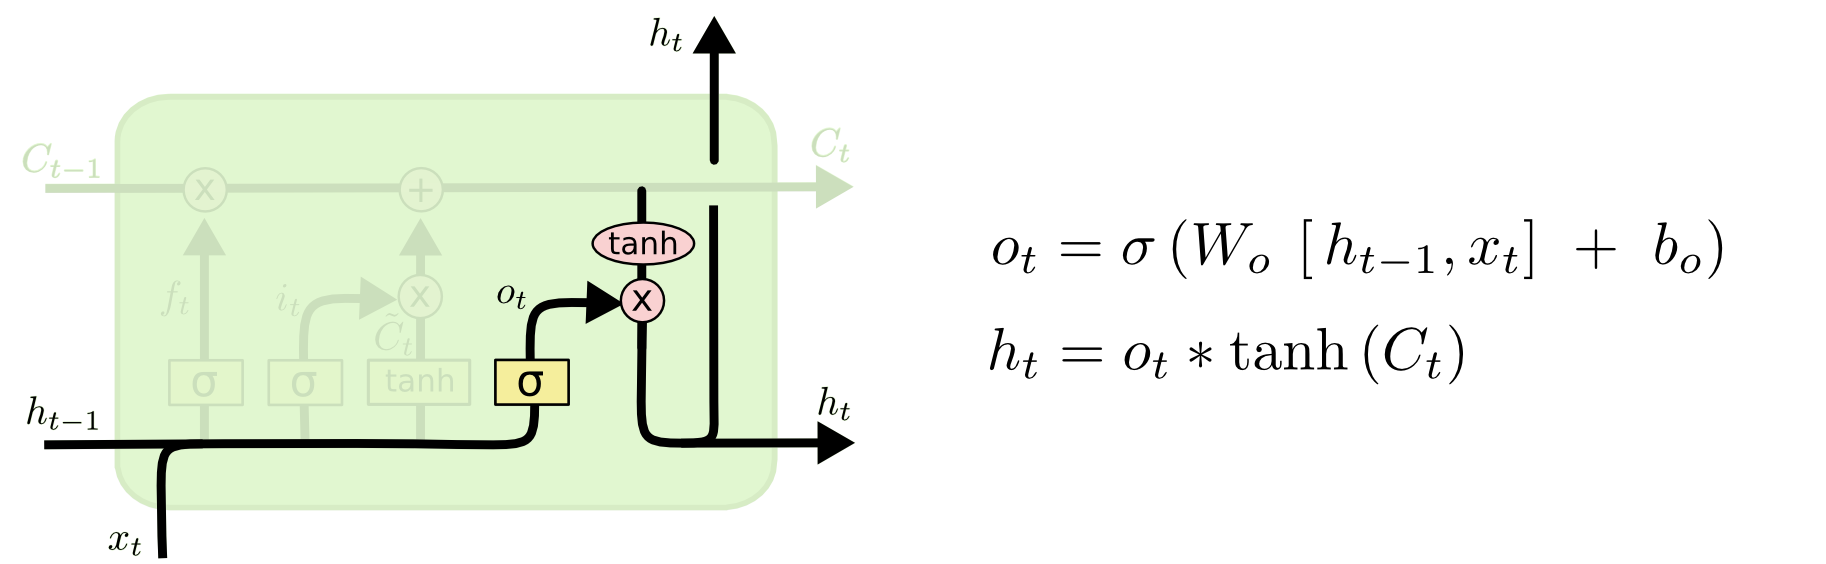
\includegraphics[width=8cm]{LSTM4.png}
	\caption{Decide the output of a LSTM network.}
	\label{fig:LSTM4}
\end{figure} 


\section{Mapping of Disease Codes}

In our word2vec approach we applied generalization on the medical states. This was needed to retrieve more general n-grams. For this generalization, we divided some attributes into specific intervals.

Instead of dividing some attributes into specific intervals, we could apply normalization to it. Based on the distribution of the data, we can make more sensible intervals and assign them to the attributes.

\section{Conclusion}
The final section of the chapter gives an overview of the important results
of this chapter. This implies that the introductory chapter and the
concluding chapter don't need a conclusion.



%%% Local Variables: 
%%% mode: latex
%%% TeX-master: "thesis"
%%% End: 
